\section{Egyszerű DNN model felépítése}

DNN alaú rendszer esetén is az első fázis a szövegből fonéma alapú címkék előállítása, ezekről részletesebben a fejezetben írtunk. Ezután meg kell határozni a fonémáknak a hosszát, erre egy egyszerű előrecsatolt háló alkalmas. Az idő paraméterekkle ellátott fonémákból becsülhetőek az aktuális időegzségre jellemző gerjesztési és spektrális paramétrek. Ezekből a paraméterekből állítható elő az eredetihez hasonloó gépi hang.

\begin{centering}
	\textbf{DNN rendszerl}\par\medskip\centering
	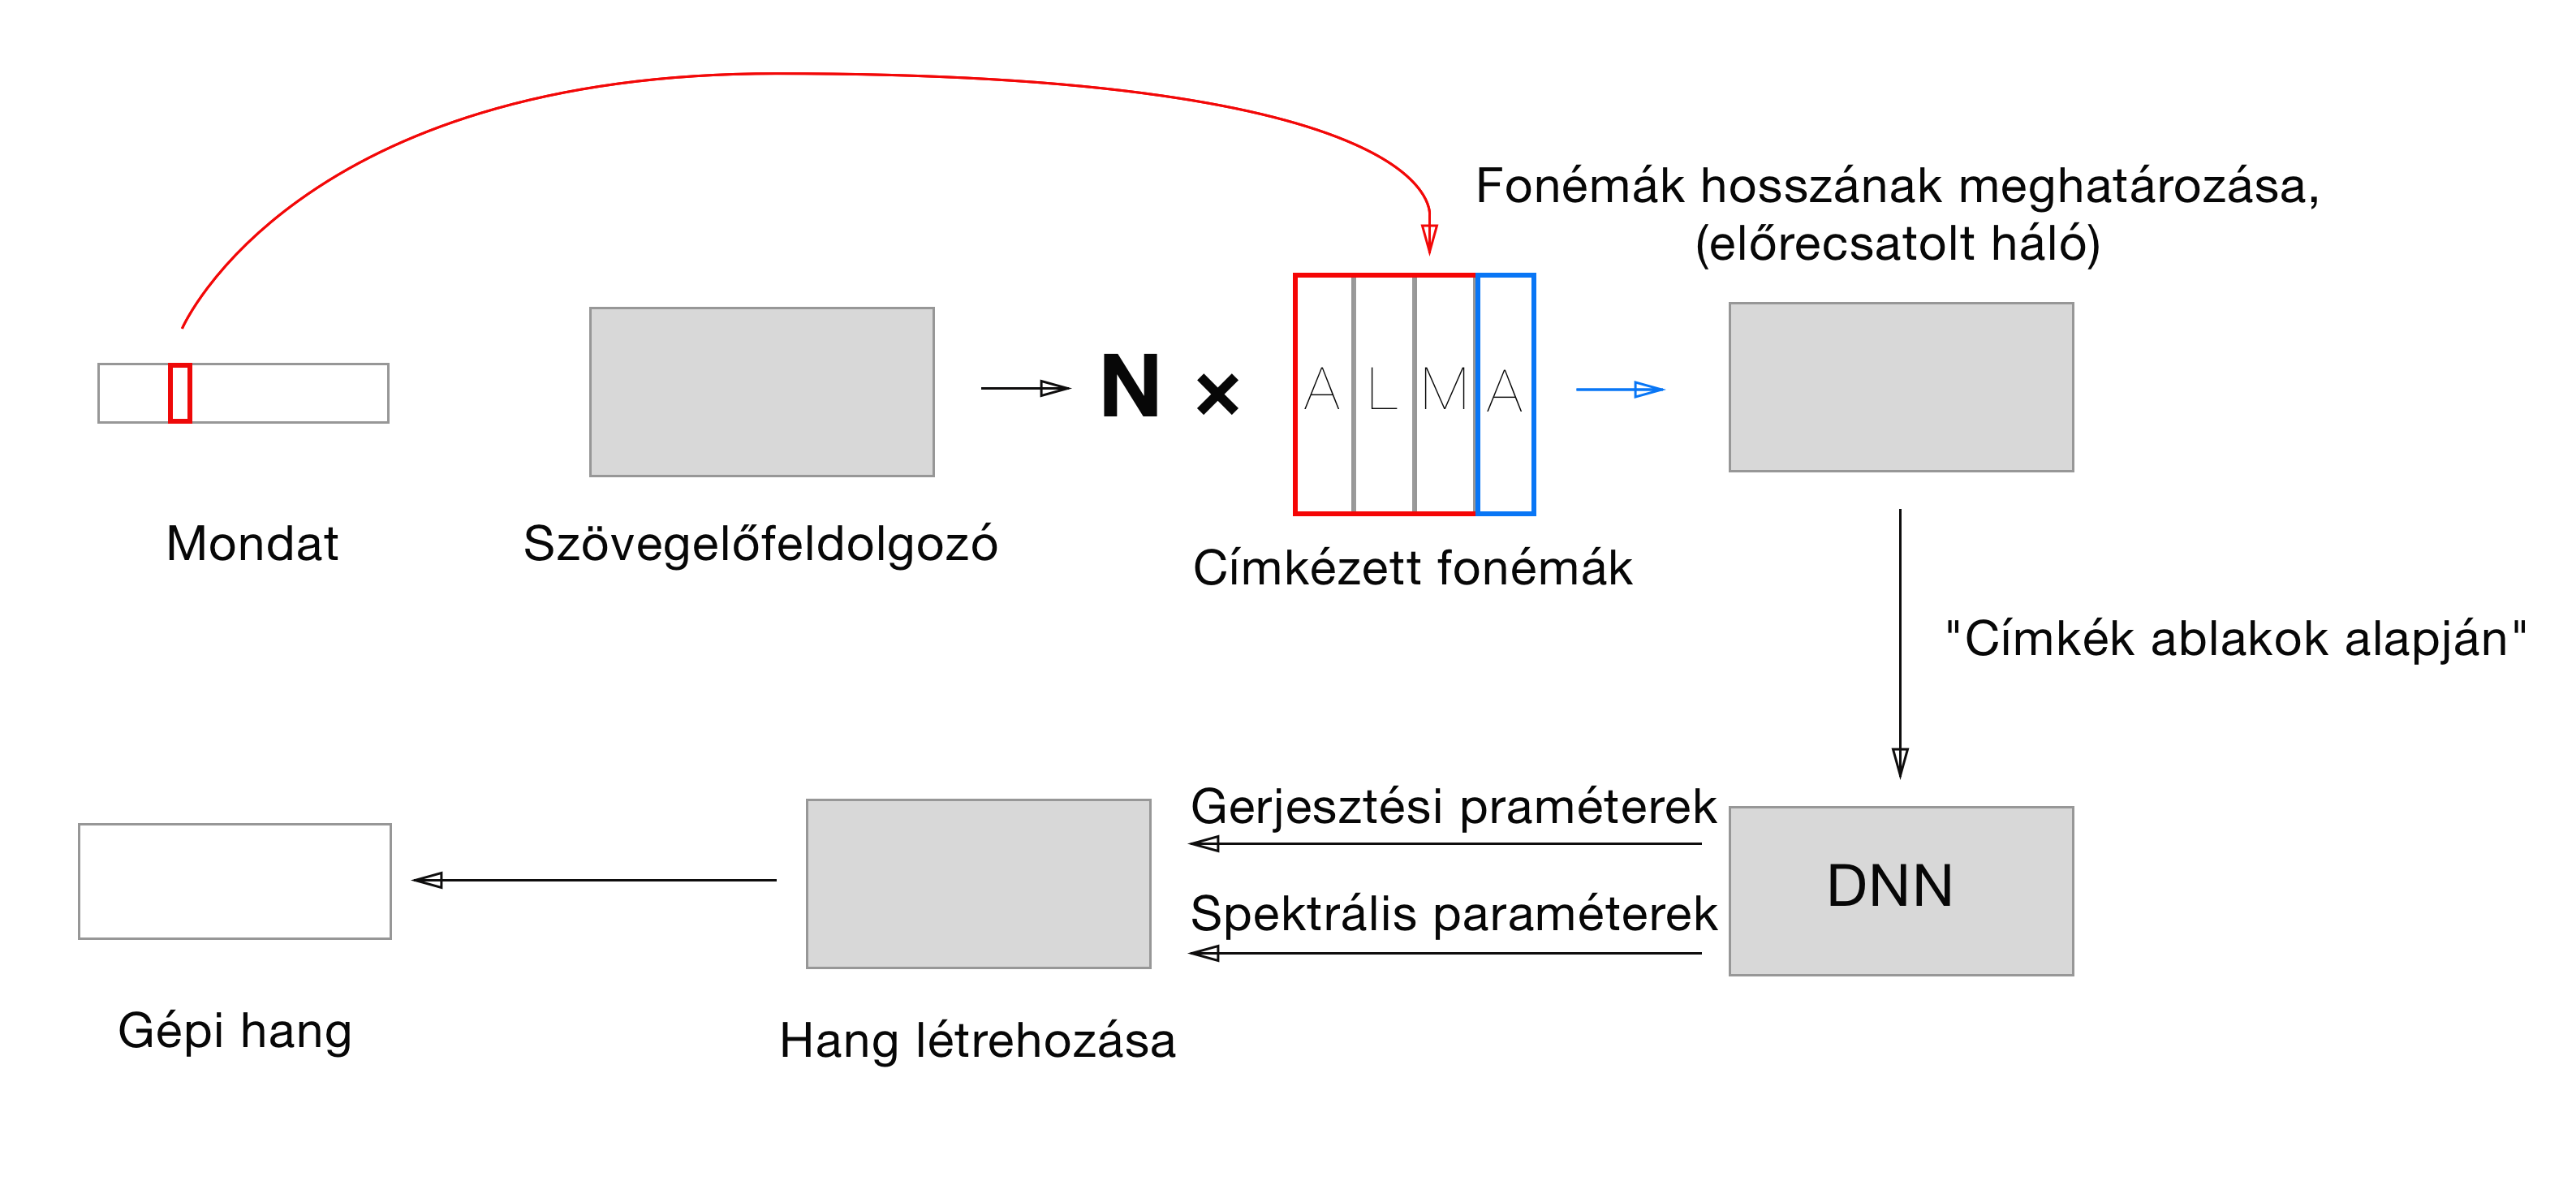
\includegraphics[width=\textwidth,keepaspectratio]{dnn_struct}
\end{centering}

\subsection{Háló modellek}
Külön hálón tanítottuk a spektrális és a gerjesztési paramétereket. 

Gerejesztési paraméter problémáját két hálóra bontottuk szét. Az egyik a hang zöngésségét határozta meg a másik pedig az alapfrekvenciát, a végleges eredményeket a két háló által jósolt értékekből számítottuk ki. (Gyakorlatilag egy engedélyező jelként értelmeztünk a zöngésség értékét az alapfrekvencián.) A zöngésség meghatározása egy egyszerűbb probléma erre  egy 6 rejtett réteget, rétegenként 512 neuront tratalmazó, RELU aktiváziós függvényt, SGD optimalizálást és MSE költségfüggvényt alkalmazó hálót hoztunk létre. Az alapfrekvencia becslésére 6 rejtett réteget, rétegenként 1024 neuront tartalmazó, tanh és sigmoid aktiváziós függvényt, SGD optimalizációt és MSE költségfüggvényt használó hálót alkalmaztunk. Utóbbi esetén a rétegenként alkalmaztunkt Dropout-ot, tanítás során pedig early stopping-ot.

A gerjesztési paramétereket meghatározó háló hasonlóan épült fel az alapfrekvenciát becslő hálóhoz, de mivel az itt elért eredményeink nem elég jó minőségűek ezen még valószinűleg változtatnunk kell.

\begin{comment}
regi reszek

A továbbiakban egy DNN model alkalmazása olvasható. A megismert cimkéket továbbiakkal egészítettük ki, majd ez alapján generáltunk gerjesztési és spektrális paramétereket, amikből előállítható az audio.





Előrecsatolt mély neurális hálózatot építettünk fel, 6 rejtett réteggel, tanh és sigmoid aktivációs függvényekkel, SGD optimalizálóval és MSE költségfüggvénnyel. A háló rétegeire Dropoutot is használtunk. (/!TODO ref)
A megállást early stoppinggal detektáltuk.

/!TODO háló modell kép

\end{comment}
